%======================================================================
\subsection{BW-ROU --- Built, 30 Oct: bend rules, one spline, BOM Length}\label{sec:rou-built-30oct}
%======================================================================

Your five answers to the open questions of Section~\ref{sec:rou-built} were built the same afternoon, in four commits:
\code{5037aaa5} ROU-02 (configurable bend rules, with the 27 Oct wire default of $4\,$OD), \code{4303defb} ROU-01
(one spline; picks clear the selection), \code{4f24234d} ROU-04 (the Assembly BOM's Length column, C++) and
\code{0429f972} (a panel fix found from the screenshot below). The maths stays FreeCAD-free in
\file{addons/BruceWorx/bruceworx/routing.py}; the objects, panels and the new dialog are in
\file{bruceworx\_routing.py} and \file{bruceworx\_routing\_gui.py}; the BOM change is in
\file{src/Mod/Assembly/App/BomObject.cpp} and \file{CommandCreateBom.py}, marked \code{[BW]}.

\begin{figure}[!htbp]
\centering
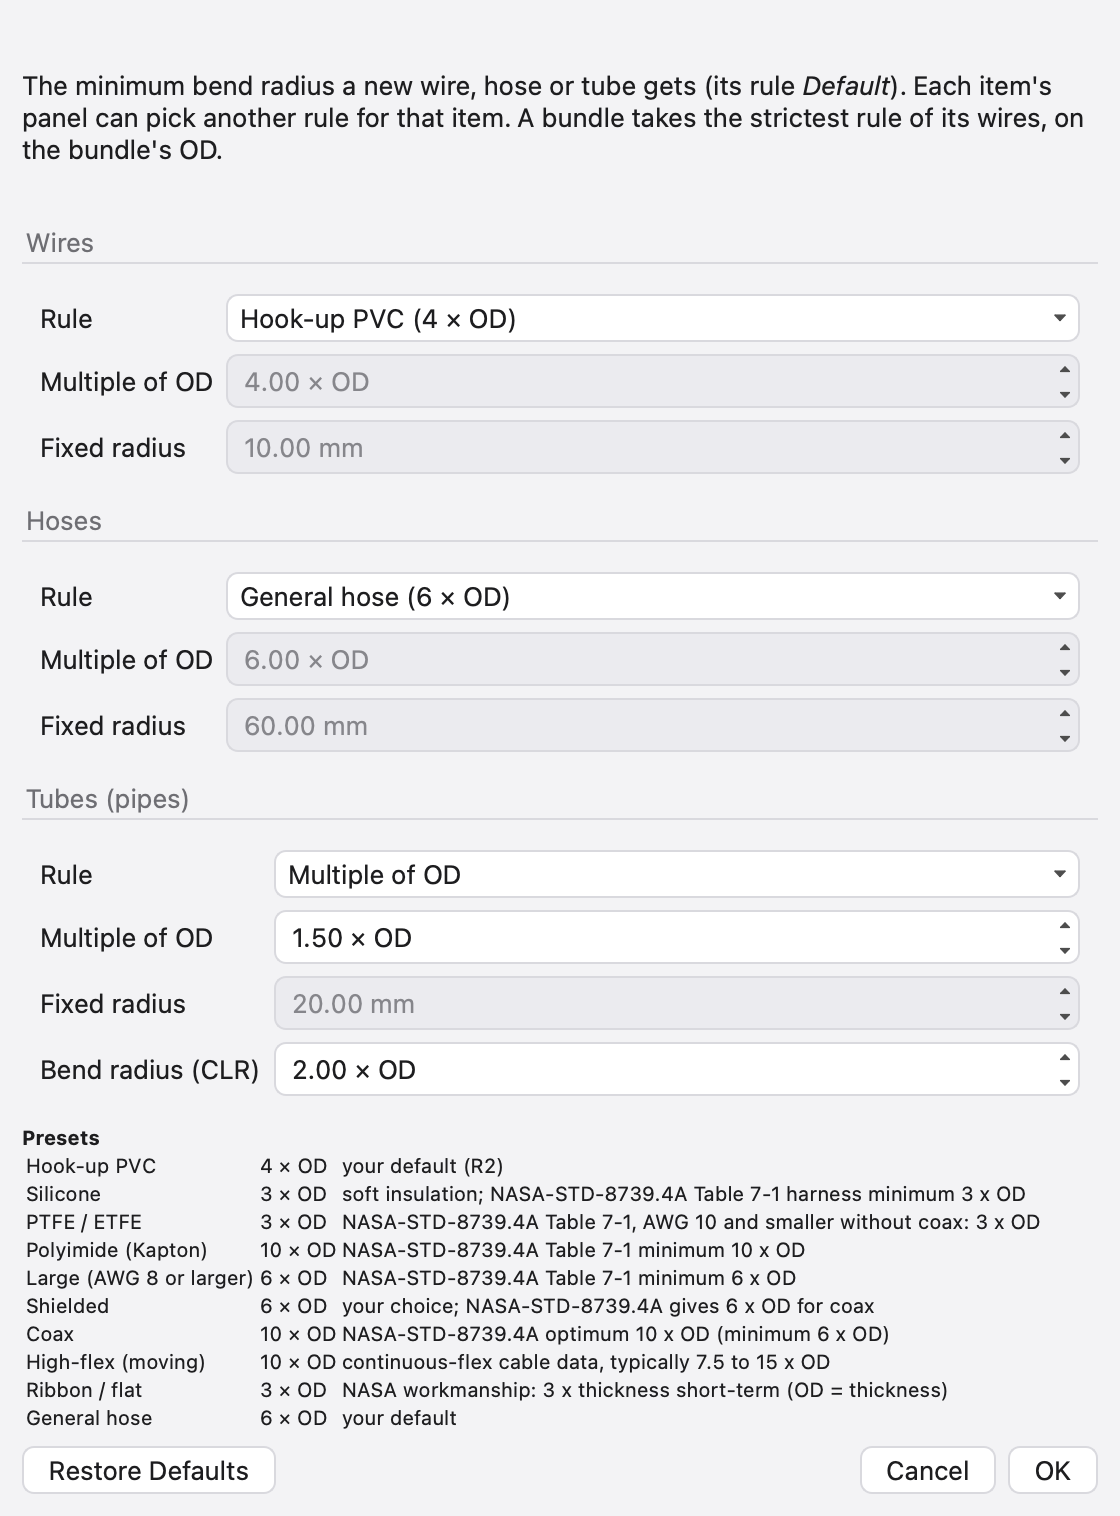
\includegraphics[width=0.52\linewidth]{fig/routing_bendrules.png}\hfill
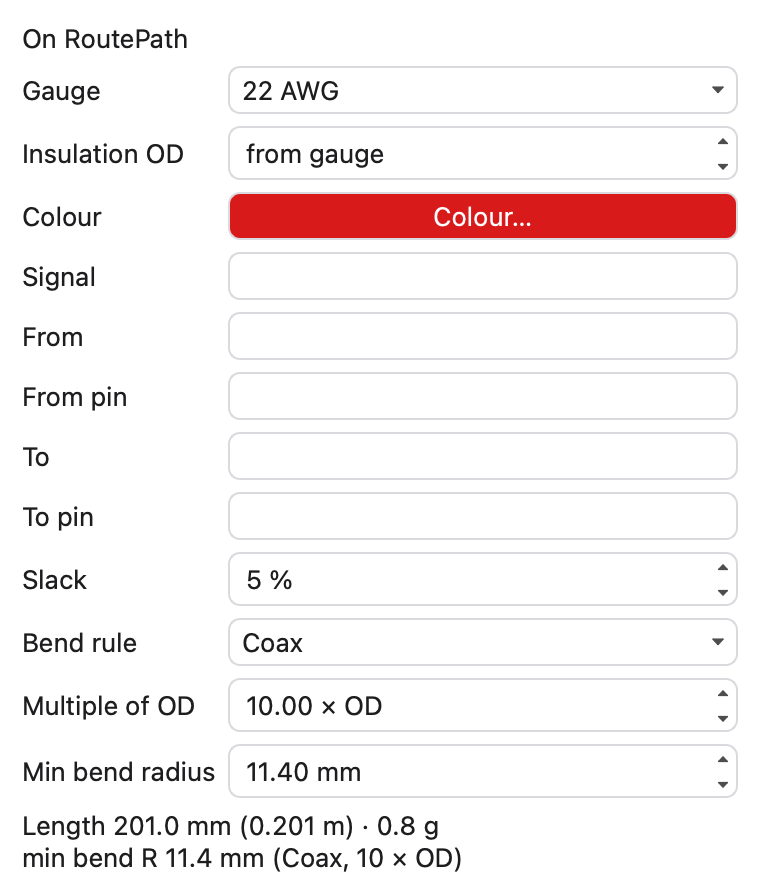
\includegraphics[width=0.40\linewidth]{fig/routing_wirepanel.png}
\caption{Left: the Bend Rules dialog (Routing tab, Items group) with the shipped defaults: hook-up PVC $4\,$OD for
wires, $6\,$OD for hoses, $1.5\,$OD minimum and $2\,$OD CLR for tubes, and the preset table with where each number
comes from. Right: a 22\,AWG wire's panel with the rule set to Coax: the minimum radius follows the insulation OD
($10 \times 1.14 = 11.4$\,mm) and the status line names the rule. Both are off-screen grabs of the real widgets.}
\label{fig:rou-built-30oct}
\end{figure}

\paragraph{What you can do now.}
\begin{itemize}[nosep]
  \item \textbf{Bend rules per item.} Every wire, hose, pipe and bundle has a \code{BendRule}: \emph{Default} (the
        preferences), a preset, \emph{Multiple of OD} (its \code{BendFactor}), \emph{Fixed radius} (its
        \code{MinBendRadius} as typed) or \emph{No check}. The item panels have the rule, the multiple and the radius;
        typing a multiple picks Multiple of OD, typing a radius picks Fixed radius (in the panel and in the property
        editor alike). \code{MinBendRadius} always holds the radius in force and \code{BendRuleUsed} says where it came
        from (``Default: Hook-up PVC, 4\,$\times$\,OD''). A rule on OD follows the OD: thicker insulation, larger radius.
  \item \textbf{Presets} (minimum radius of a static, installed bend):
        \begin{center}\small
        \begin{tabularx}{\linewidth}{@{}llX@{}}
        \toprule
        Preset & Rule & Source \\
        \midrule
        Hook-up PVC (default) & $4\,$OD & your R2 \\
        Silicone & $3\,$OD & your suggestion; NASA-STD-8739.4A Table 7-1, harness without coax, minimum $3\,$OD \\
        PTFE / ETFE & $3\,$OD & NASA-STD-8739.4A Table 7-1 (AWG 10 and smaller, no coax) \\
        Polyimide (Kapton) & $10\,$OD & NASA-STD-8739.4A Table 7-1 (optimum $15\,$OD) \\
        Large (AWG 8 or larger) & $6\,$OD & NASA-STD-8739.4A Table 7-1 \\
        Shielded & $6\,$OD & your suggestion \\
        Coax & $10\,$OD & your suggestion; NASA-STD-8739.4A optimum $10\,$OD, minimum $6\,$OD \\
        High-flex (moving) & $10\,$OD & continuous-flex cable data, typically 7.5--15\,$\times$\,OD \\
        Ribbon / flat & $3\,$OD & NASA workmanship guidance: $3\times$ thickness short-term ($10\times$ long-term) \\
        General hose (default) & $6\,$OD & your default \\
        \bottomrule
        \end{tabularx}
        \end{center}
  \item \textbf{Defaults in one place.} \textbf{Bend Rules} (a new button in the Routing tab's Items group) sets the
        default rule for wires, hoses and tubes (a preset, a multiple, a fixed radius or no check) and the tube CLR
        multiple, in the preference group \code{Mod/BruceWorx/Routing} (\code{WireRule}, \code{WireFactor},
        \code{WireRadius}, the same for \code{Hose} and \code{Tube}, and \code{TubeClrFactor}). OK recomputes every
        open item that follows the defaults; Restore Defaults puts the shipped values back.
  \item \textbf{Bundles} take the strictest rule of their wires (\emph{From wires}) unless set: a multiple of OD is
        taken of the bundle's own OD (as NASA-STD-8739.4A states harness radii on the overall OD), a fixed radius as
        it is. Three 1.6\,mm hook-up wires make a 3.19\,mm bundle with a 12.7\,mm minimum; make one of them Coax and
        it is 31.9\,mm.
  \item \textbf{One spline.} A Spline-mode path is drawn from the module's own spline (C2 cubic, not-a-knot ends,
        chord-length parameters), built exactly as a clamped cubic B-spline: degree 3, knots at the chord parameters,
        $n+2$ poles for $n$ points. The length and tightest radius in the panel are those of the drawn curve. Nine
        points on a semicircle of $R=50$ now draw and check at 45.8 (before, the OCC curve was drawn and checked
        at 44.9 while the module said 45.8); thirteen on $R=100$ give 95.7.
  \item \textbf{Picks clear the selection.} In the Route Path panel each pick becomes a point and the selection is
        cleared, as Fusion's point tools do; so are the picks the panel opens with and Add selection.
  \item \textbf{Assembly BOM Length.} The Bill of Materials has an automatic \emph{Length} column, on by default for
        new BOMs and offered as ``Length (auto)'' in the panel's Add column menu: for a wire, pipe or hose it prints
        Quantity $\times$ \code{QuantityPer} with \code{QuantityUnit} (a hose used twice at 0.21\,m reads
        ``0.42\,m'', a link array of three plus one at 0.25\,m reads ``1\,m''); counted parts stay blank. The
        RoutePath is no longer a BOM line.
\end{itemize}

\paragraph{Decided while building.}
\begin{itemize}[nosep]
  \item \textbf{A rule is a choice plus two numbers}, not a parsed string: \code{BendRule} (an enumeration),
        \code{BendFactor} and \code{MinBendRadius}. \code{MinBendRadius} stays the one property everything checks
        against, so the Browser badge, the reports and scripts did not change.
  \item \textbf{Migration of 27 Oct documents} (on load, before the first recompute): a wire with a radius typed in
        keeps it as a fixed override; a wire without one takes the Default rule, so old wires are now checked at
        $4\,$OD (they were not checked before, as you decided); a hose or pipe at its old default ($6\,$OD, $1.5\,$OD)
        becomes Multiple of OD with that factor, so it keeps its value and keeps following OD; any other radius is a
        fixed override; zero is No check. A bundle with no radius is From wires.
  \item \textbf{The exact B-spline.} Each segment's Bézier points are $\mathbf P_i + \tfrac h3\mathbf r'$ and
        $\mathbf P_{i+1} - \tfrac h3\mathbf r'$; for a C2 spline they lie on the legs of one control polygon, each
        leg cut in the ratio $h_{i-1}:h_i:h_{i+1}$ of the neighbouring spans, so the polygon is read off by extending
        each segment's middle leg. No knot removal and no approximation; the not-a-knot condition only means two of
        the knots could be removed, and keeping them is harmless.
  \item \textbf{Skipping paths uses a property}, \code{BomExclude} (hidden, true on every RoutePath, added to old
        paths on load), so the C++ BOM does not need to know BruceWorx's Python types; the vault BOM walker keeps
        skipping by type as before.
  \item \textbf{The Length cell is text} (``0.42 m'' with the sheet's leading quote), three decimals with trailing
        zeros dropped, so the spreadsheet does not turn it into a unit expression.
\end{itemize}

\paragraph{Tests.} Unit (\file{test\_routing.py}, 28): six new for the rules (radius and text, the presets, defaults
from preferences including an unknown name, item rules, a bundle's strictest rule, migration) and one checking the
B-spline against the spline on five point sets (de~Boor, $10^{-9}$). Headless (\file{TestBruceWorxRoutingCore.py},
17): per-item rules (Default $4\,$OD, Coax following the OD, a typed radius, a typed multiple, No check, hose and
tube defaults, CLR $2\,$OD), the preferences driving the defaults, a bundle's strictest wire, 27 Oct items saved and
reloaded (five cases), the Part edge's knots, points, first derivatives and curvature equal to the module's, the
semicircle, and the Assembly BOM's Length column on a real hose with its path skipped. Assembly
(\file{TestAssemblyWorkbench}, 44, three new in \file{TestBWBom.py}: the Length column with a link, a link array and
an empty unit; \code{BomExclude}). GUI (\file{TestBruceWorxRouting.py}, 9): the pick test now checks the selection is
empty after each pick; the wire panel's rule, preset and typed multiple; the hose panel's typed radius; the Bend
Rules dialog writing the preferences and recomputing a following wire, a fixed wire and a hose, Restore Defaults; the
BOM panel's default Length column. \file{TestBruceWorxWorkspaces} (25), \file{TestBruceWorx} (15) and
\file{TestBruceWorxBom} (4) pass.

\paragraph{Sources.} NASA-STD-8739.4A with Change 4, \emph{Crimping, Interconnecting Cables, Harnesses, and Wiring},
Table 7-1 ``Bend Radii for Completed Interconnecting Cable or Harness'' (read from the standard itself). NASA's
workmanship pages for flat and ribbon cable ($3\times$ short-term, $10\times$ long-term), from a search summary.
IPC/WHMA-A-620 Table 14-1 (by revision) has per-class radii for unshielded, shielded and coax cable; I could not
read the table itself, so no preset cites it. FAA AC~43.13-1B Chapter 11 gives bundles $10\times$ the largest wire's
OD ($3\times$ where supported), as quoted by secondary sources.

\paragraph{Open questions for you.}
\begin{enumerate}[nosep]
  \item \textbf{A bundle's rule}: the strictest wire rule on the \emph{bundle's} OD (NASA's way, built), or the
        aircraft way, $10\times$ the \emph{largest wire's} OD (AC~43.13-1B)? The two differ by about $3\times$ on a
        small harness.
  \item \textbf{PTFE/ETFE at $3\,$OD and High-flex at $10\,$OD} are my picks. If you have IPC/WHMA-A-620 at hand,
        should its Table 14-1 classes replace them (and add Class 2/3 as a choice)?
  \item \textbf{Hoses} have one preset. Hydraulic hose radii come per dash size from the catalogue (SAE~J517 /
        ISO~18752); add a table by size, or is Fixed radius per hose enough?
  \item \textbf{Old wires are now checked at $4\,$OD}, so a 27 Oct harness may show new ``bend too tight'' badges.
        Fine, or migrate unset wires to No check?
  \item \textbf{Existing BOMs} keep their columns; only new ones get Length. Add it to existing BOMs on load?
\end{enumerate}
